\documentclass[justified]{tufte-handout}
\usepackage{../braph2_tut}
%\geometry{showframe} % display margins for debugging page layout

\title{Pipeline for Comparison of Connectivity Data using Binary Undirected graphs at fixed Thresholds}

\begin{document}

\maketitle

\begin{abstract}
\noindent
In this tutorial, we will upload a file containing the pipeline with the different steps to compare two groups of subjects using \emph{connectivity data} (check tutorial \emph{Group of Subjects with Connectivity Data}) and binary undirected graphs at fixed thresholds. This Tutorial explains how to perform group analyses and comparisons with this kind of data.
\end{abstract}

\tableofcontents

\fig{figure*}
	{fig:01}
	{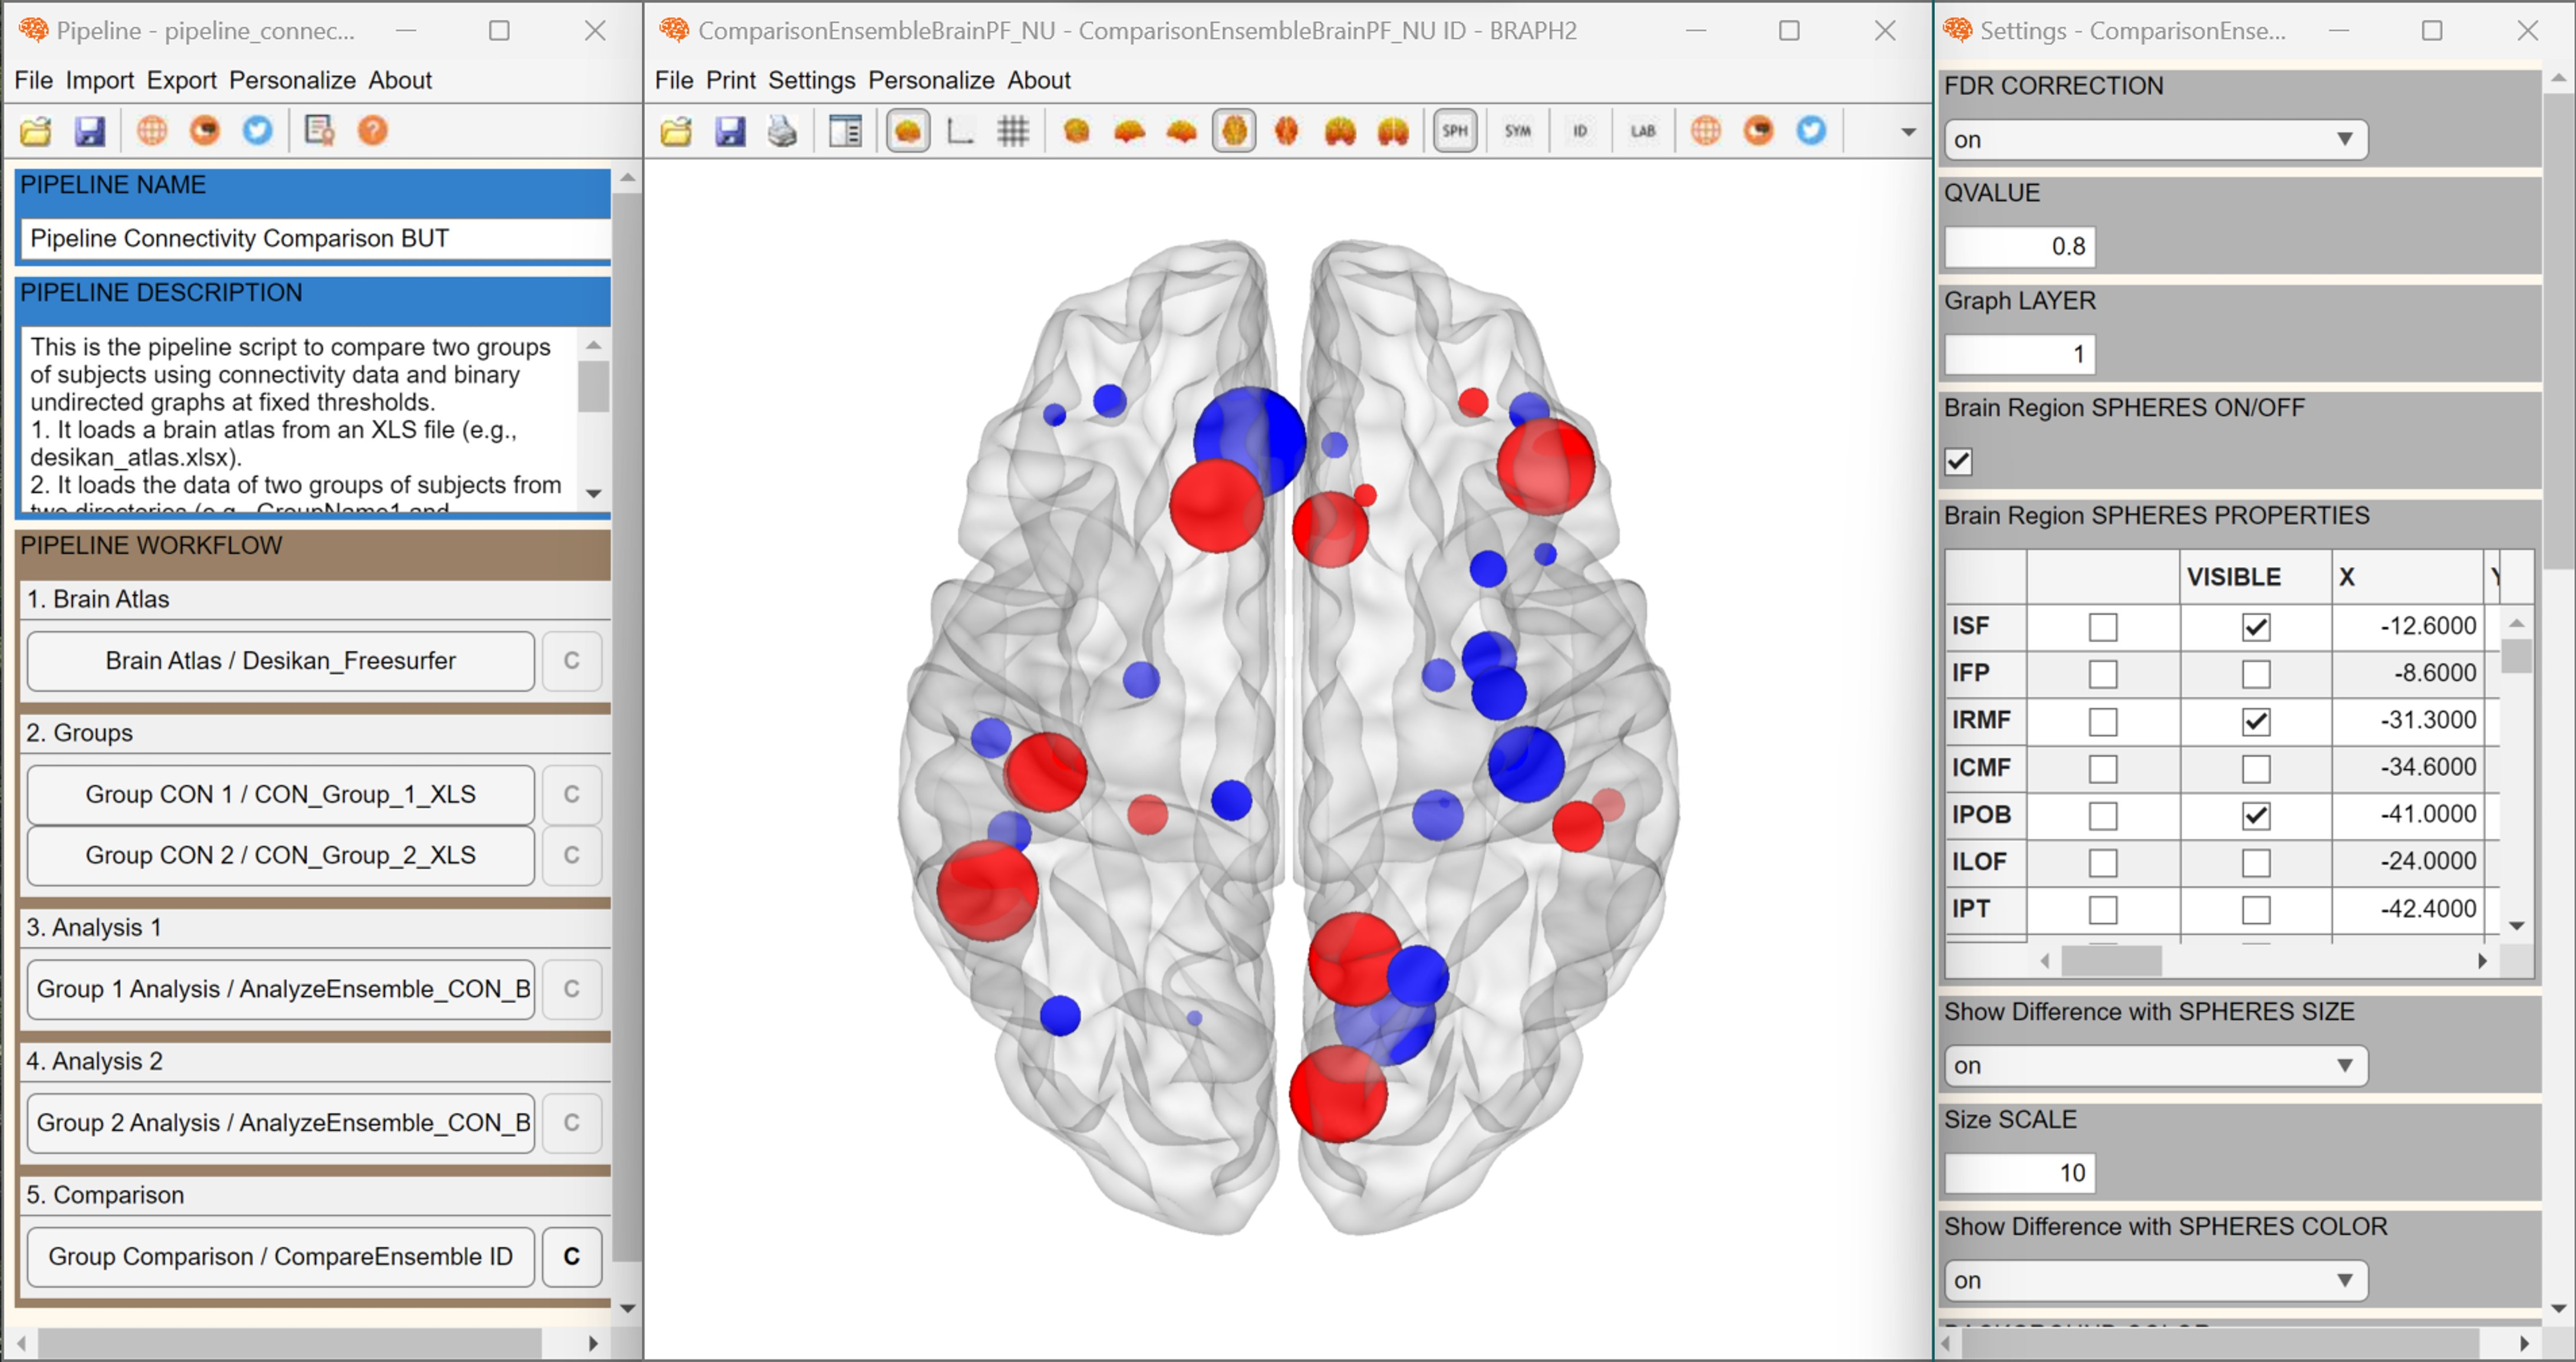
\includegraphics{fig01.jpg}}
	{GUI for working with the pipeline to compare two groups of subjects with \emph{connectivity data} using binary undirected graphs at fixed thresholds}
	{
	Full graphical user interface to perform group comparisons with \emph{connectivity data} in BRAPH~2.0. 
	}

\clearpage
\section{Open the GUI}

The pipeline GUI can be opened by typing \code{braph2} in MatLab's terminal, which allows you to select a pipeline, in this case, \fn{pipeline\_connectivity\_comparison\_but.braph2} (containing the steps required to perform your analysis).

To open the GUI and upload the connectivity comparison pipeline, you can also do it from the command line by typing the commands in \Coderef{cd:launch}.
%
\begin{lstlisting}[
	label=cd:launch,
	caption={
		{\bf Code to launch the GUI to upload a pipeline file to compare two groups of subjects.}
		This code can be used in the MatLab command line to launch the GUI to upload a pipeline file.
	}
]
pip = Pipeline(); ¥\circled{1}\circlednote{1}{creates a new object \code{Pipeline} to upload the steps to perform an analysis or comparison.}¥

gui = GUIElement('PE', pip); ¥\circled{2}\circlednote{2}{creates a GUI to upload the files into the pipeline.}¥
gui.get('DRAW')¥\circled{3}\circlednote{3}{draws the GUI.}¥
gui.get('SHOW') ¥\circled{4}\circlednote{4}{shows the GUI.}¥
\end{lstlisting}

Once the pipeline is uploaded, you can see a GUI that contains different steps: to upload a brain atlas, to upload the connectivity data of two groups, analyze them, and finally, to compare the groups (\Figref{fig:02}a). 

\section{Step 1: Load the Brain Atlas}
\Figref{fig:02} shows how to upload and plot the brain atlas that you used to extract the \emph{connectivity data} for your analysis. For more information on where to find different atlases or how to change plotting settings on the brain surface, check the \emph{Brain Atlas} tutorial.

\fig{figure*}
	{fig:02}
	{
	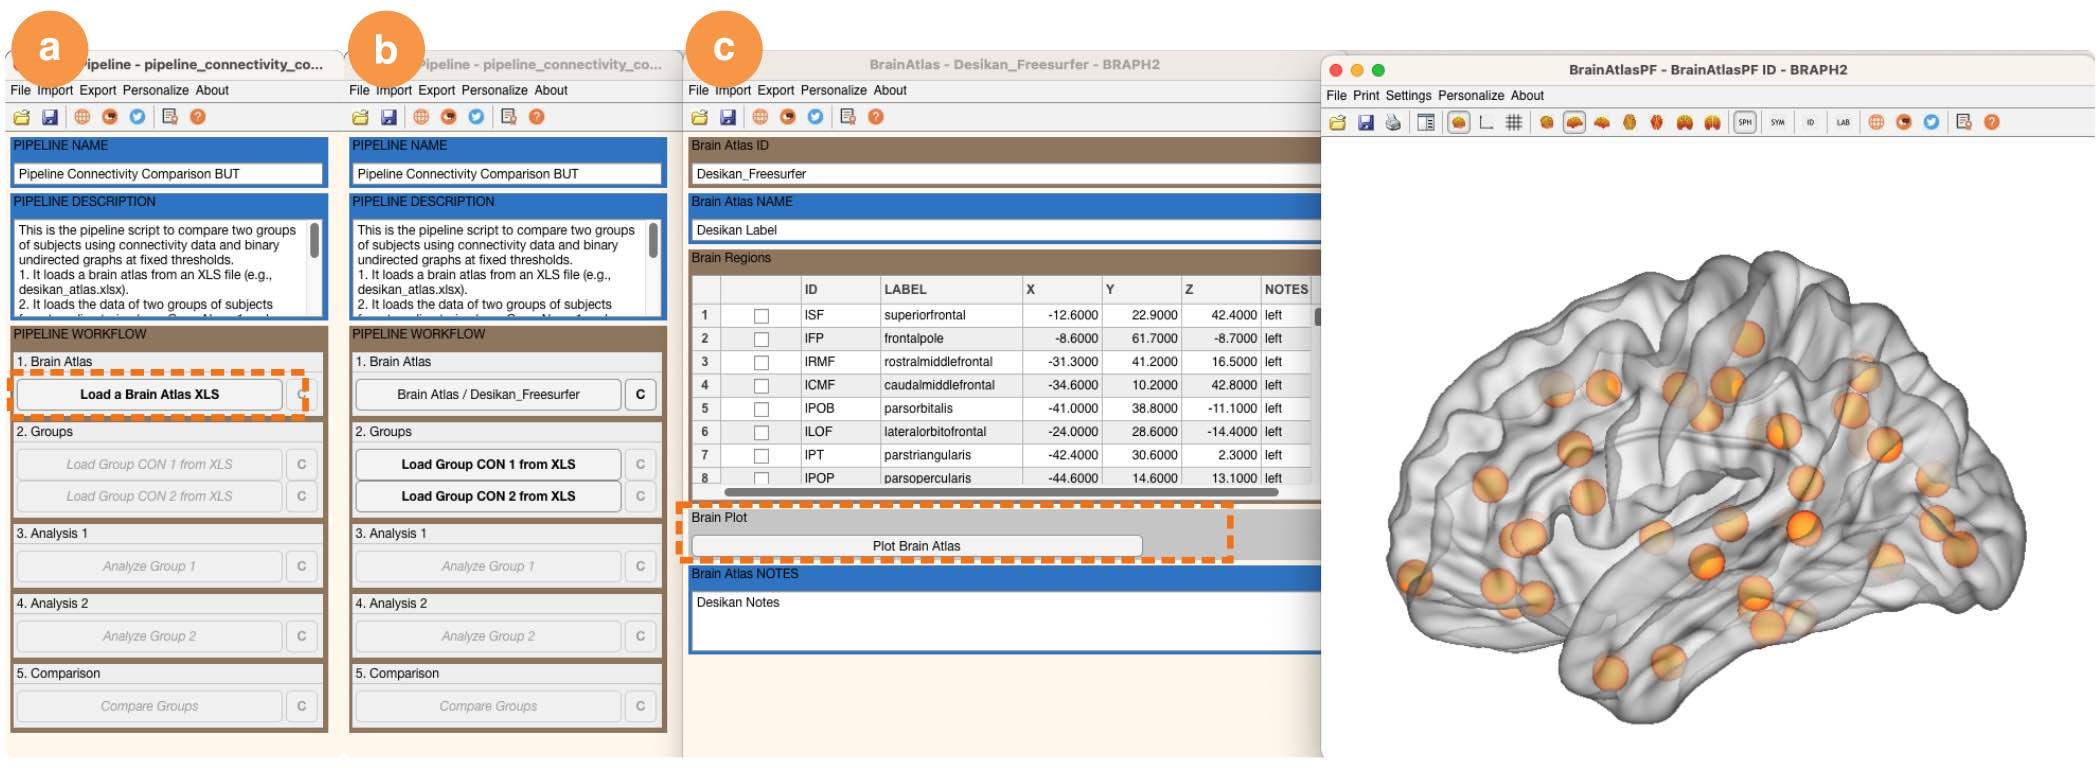
\includegraphics{fig02.jpg}
	}
	{Uploading the Brain Atlas}
	{
	Steps to upload the brain atlas:
	{\bf a} Click on \fn{Load Atlas} from the pipeline GUI.
	{\bf b} Navigate to the BRAPH~2.0 folder \fn{atlases} and select one of the atlas files, in this example the \fn{desikan\_atlas.xlsx}. {\bf c} You can also plot the brain atlas by pressing \fn{Plot Brain Atlas}. 
	}
 
\section{Step 2: Load the Connectivity Group Data}

After you loaded the brain atlas, you can upload the \emph{connectivity data} for each group as shown in \Figref{fig:03}. A new interface will be shown containing the data for the group you just selected. You can open each subject’s connectivity matrices by selecting the subject, right click, and select “Open selection” (for more information check tutorial \emph{Group of Subjects with Connectivity Data}).
	
	\fig{figure}
	{fig:03}
	{
	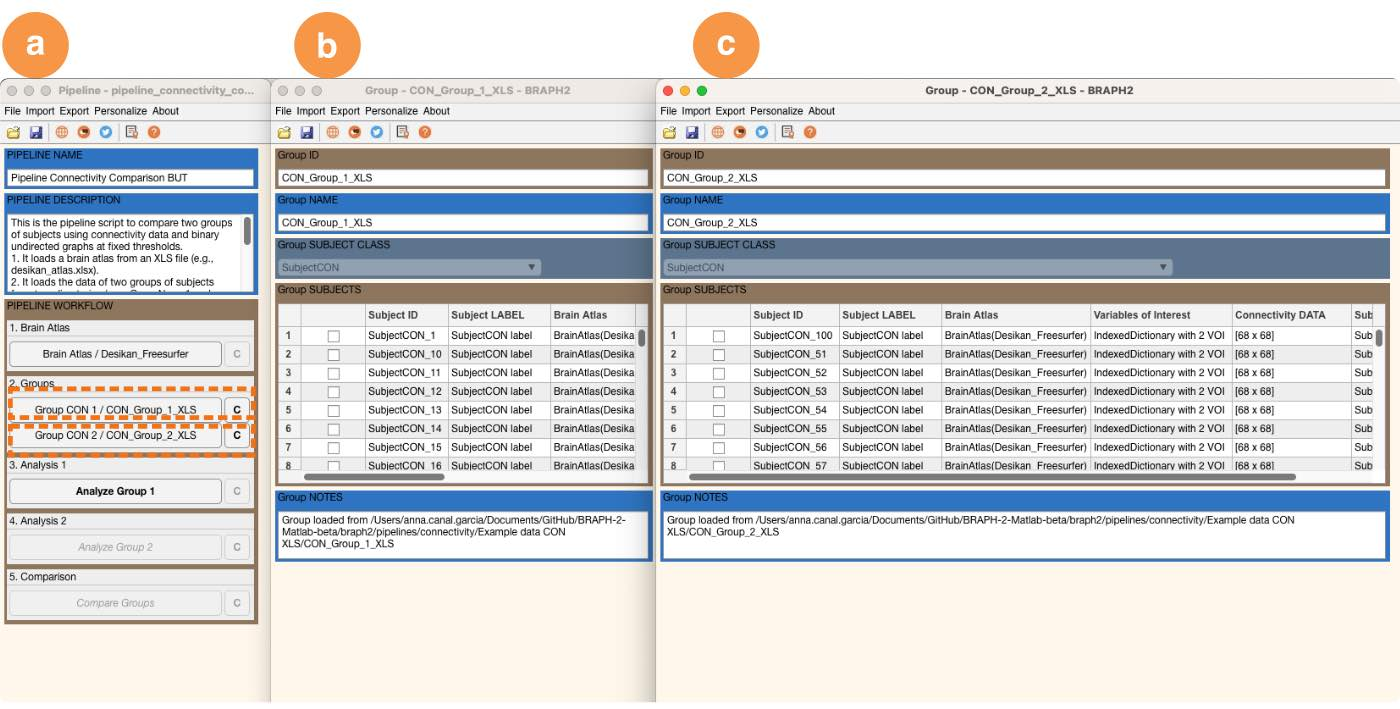
\includegraphics{fig03.jpg}
	}
	{Loading the Groups Data}
	{
	{\bf a} From the pipeline GUI, click on \fn{Load Group CON 1 from XLS} to load the data of group 1, and \fn{Load Group CON 2 from XLS} to load the data of group 2.
	{\bf b} Data for group 1 is uploaded. {\bf c} Data for group 2 is uploaded.
	}

\section{Step 3: Analyzing the Data of Group 1}

Once you have loaded the data for both groups, you can begin analyzing the data for your first group by clicking on \fn{Analyze Group 1} (\Figref{fig:04}a). 
This action will open a new interface called \fn{Analyze Ensemble}, which allows you to pre-calculate network measures for each group and explore them. 
Before these network measures are calculated, it is important to ensure two key aspects: (1) the measures are configured with the rules or parameters you desire (note that not all measures have rules or parameters), and (2) the graph is constructed based on the specified thresholds.

Importantly, the parameters you select for this analysis, including both graph and measures parameters, will remain fixed for the analysis of the second group and for group comparisons. Let's guide you through the process of preparing these parameters for both measures and graphs.

\subsection{Setting Rules for Measures}

To configure the measures, start by clicking on \fn{Graph Template} (\Figref{fig:04}b). This will open a new interface for graph template settings. 
Scroll down to find the \fn{Graph MEASURES} section. 
By clicking the 'C' button, all compatible measures will be displayed in a table. 
For example, you can select the \fn{Community Structure} measure and then right-click at the top of the table (\Figref{fig:04}c). 
In the right-click menu, choose “Data Selected Measures.” 
This will open the measure window, allowing you to specify the rules or parameters (\Figref{fig:04}d).

\subsection{Setting Parameters for Graphs}

After configuring the rules for the measures, return to the \fn{Analyze Ensemble} interface (\Figref{fig:04}e). 
In the \fn{THRESHOLDS} section, you can define the thresholds by entering values like “[0.4 0.5 0.6 0.7]” or “0.4:0.1:0.7”. 
In this tutorial, we will stick with the default thresholds. 
In brain connectivity analysis, threshold values dictate the required connection strength between different brain regions for them to be considered “connected” in a binary undirected graph. 
Adjusting these thresholds allows you to explore varying levels of brain connectivity, providing insights into how regions communicate at different threshold settings.

\fig{figure}
{fig:04}
{
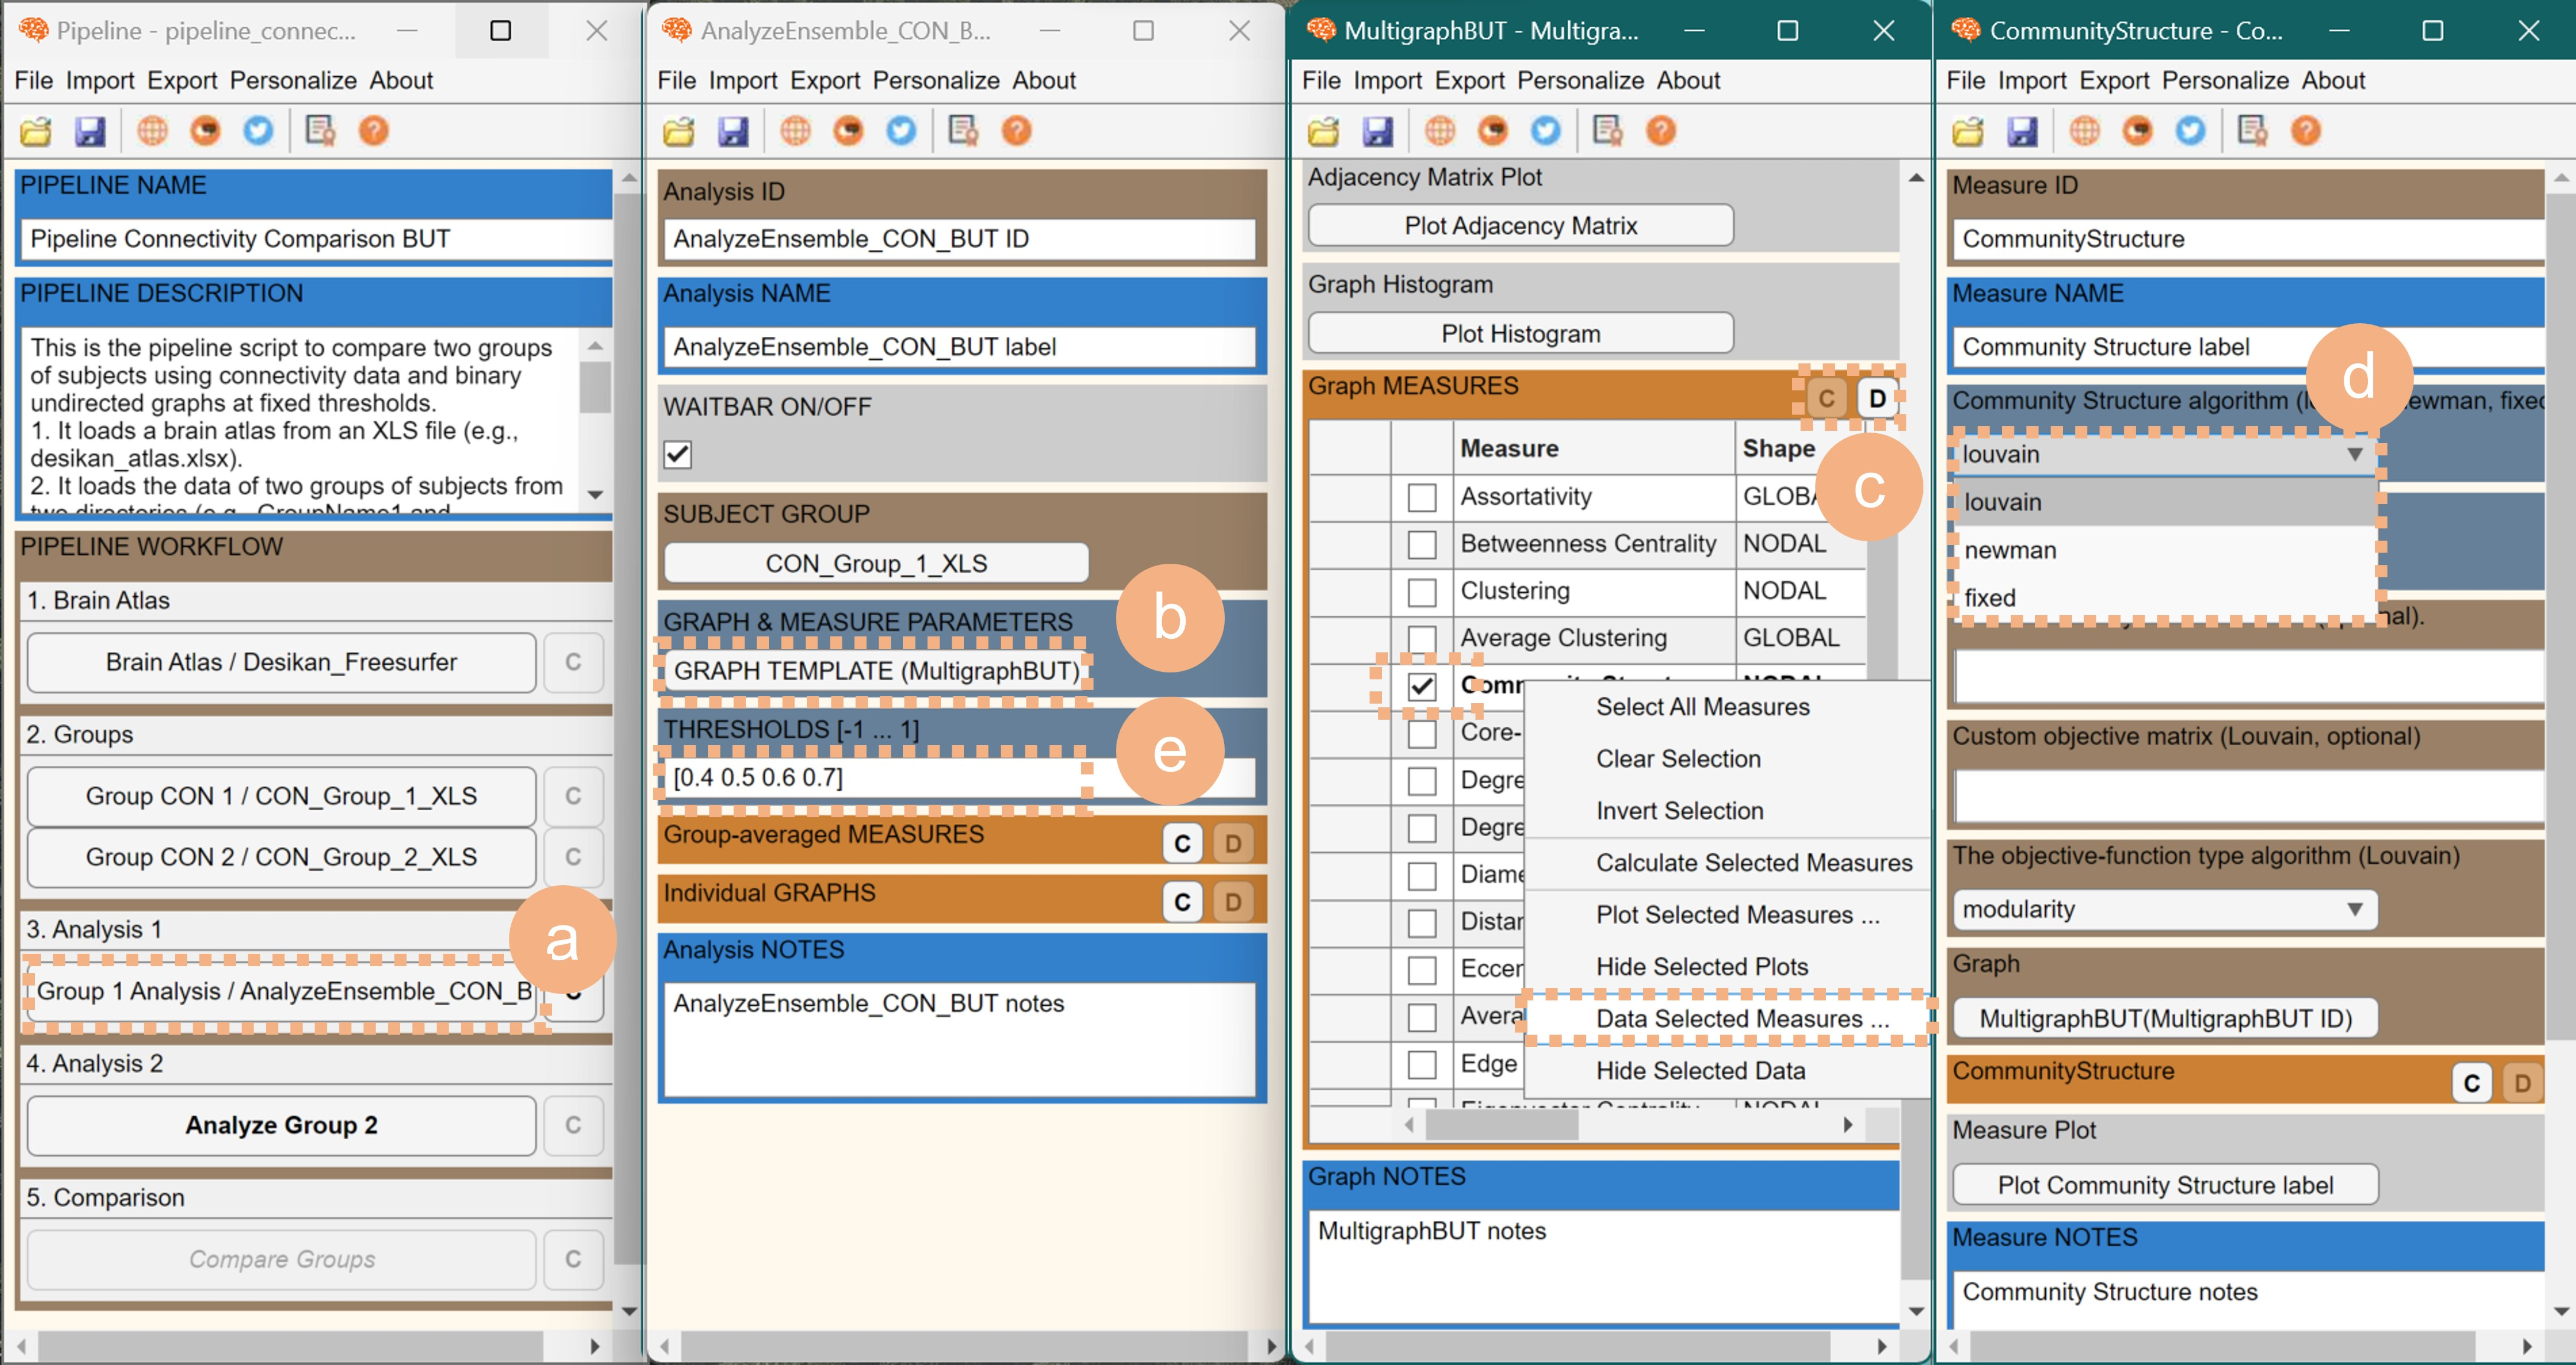
\includegraphics{fig04.jpg}
}
{Configuring Measure Rules and Parameters Before Calculation}
{
{\bf a} To initiate the analysis of data for group 1, click on \fn{Analyze Group 1}.
{\bf b} Access the graph template settings by clicking on \fn{GRAPH TEMPLATE}, opening a new interface.
{\bf c} Inside this interface, you'll find the \fn{Graph MEASURES} panel. Click the 'C' button to reveal a table displaying all compatible measures. Select the \fn{Community Structure} measure and then right-click at the top of the table. In the right-click menu, choose “Data Selected Measures.”
{\bf d} The measure window that opens allows you to define the rules or parameters for the \fn{Community Structure} measure.
{\bf e} After configuring the measure rules, return to the \fn{Analyze Ensemble} interface to set the thresholds.
}

	
\fig{figure}{fig:05}{
	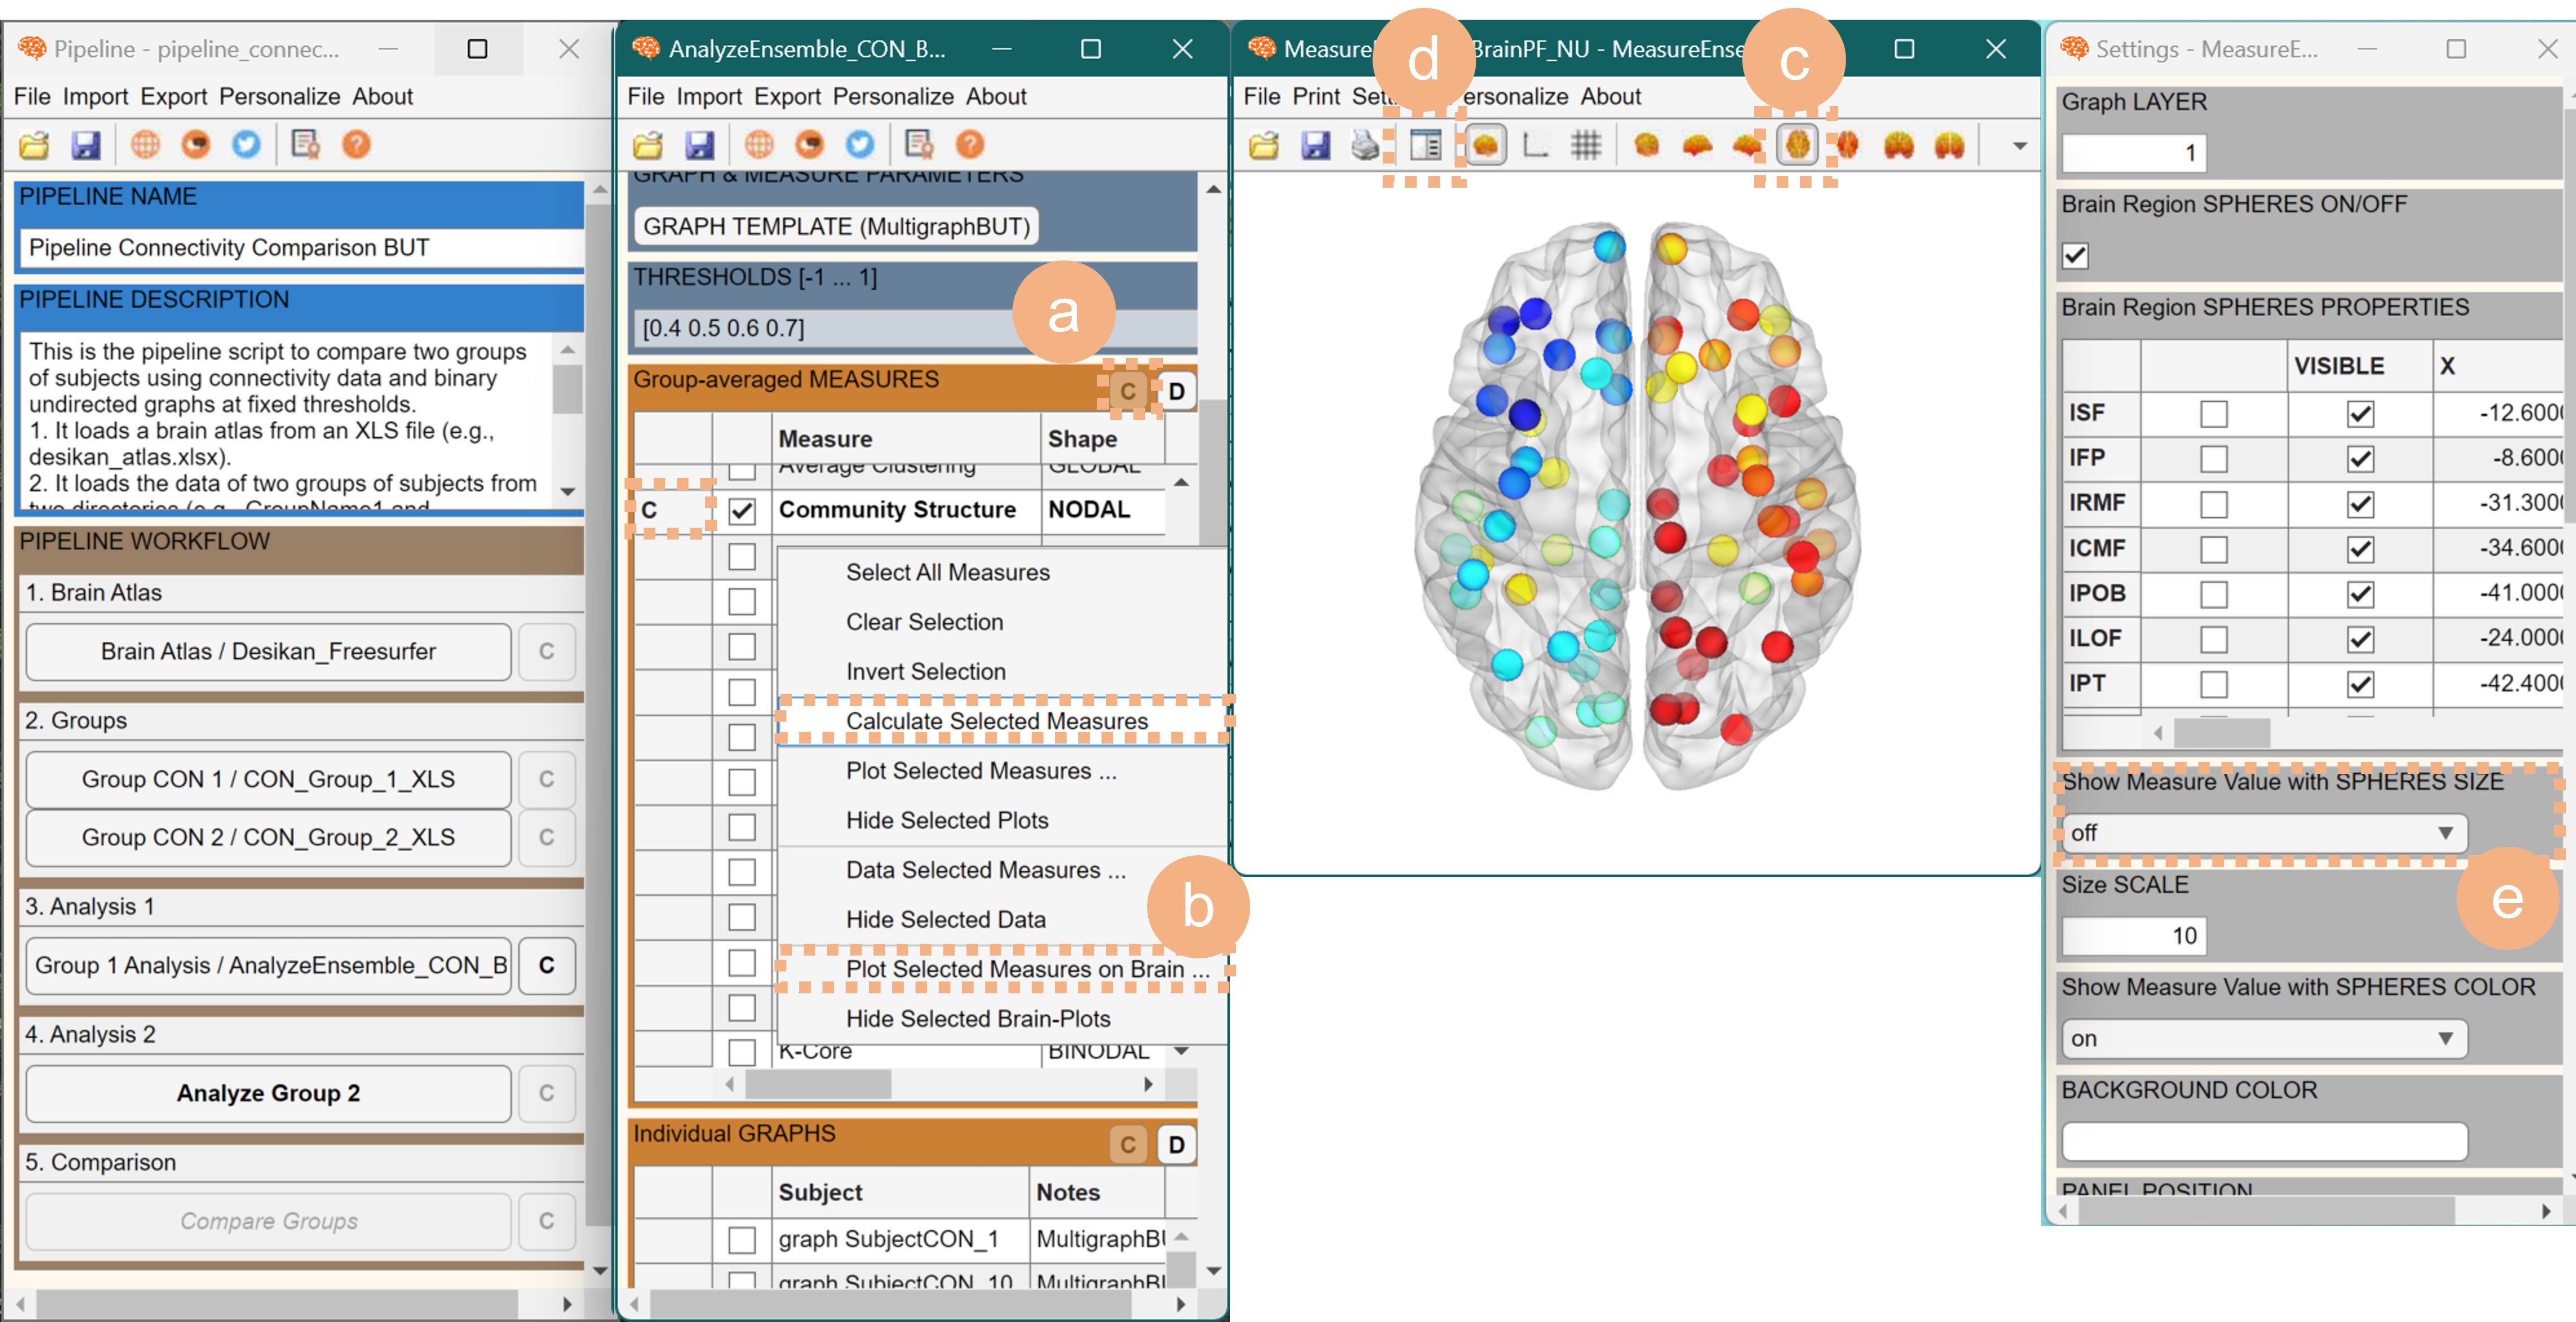
\includegraphics{fig05.jpg}
}{Analyzing the Group Data}{
	{\bf a} Locate the \fn{Group-averaged MEASURES} panel and click the 'C' button to 		reveal a table of compatible measures. Choose the \fn{Community Structure} measure, right-click it, and select “Calculate Selected Measures” to perform the calculation.
	{\bf b} To visualize the results, right-click at the top of the table and choose \fn{Plot Selected Measures on Brain} in the Analyze Ensemble interface. This action opens a brain surface with the \fn{Community Structure} plotted.
	{\bf c} Explore different views by clicking the “Axial dorsal” button in the brain surface toolbar.
	{\bf d} Adjust visualization settings by clicking on the “Settings Panel Figure” button in the same toolbar.
	{\bf e} Customize and save plot visualizations within the settings menu.
}
 
After configuring these parameters, you can proceed to calculate specific graph measures (\Figref{fig:05}). To do this, return to the \fn{Analyze Ensemble} interface (\Figref{fig:05}a) and scroll down to locate the \fn{Group-averaged MEASURES} panel. By clicking the 'C' button, you will see a table displaying all compatible measures.

As an illustrative example, let's select the \fn{Community Structure} measure, for which we previously set the rule to \fn{louvain}. Right-click at the top of the table and choose “Calculate Selected Measures.” Once the calculation is complete, you will notice a \fn{C} appearing in front of the \fn{Community Structure}, indicating that this measure has been calculated.

If you wish to visualize the results, right-click at the top of the table and select \fn{Plot Selected Measures on Brain} within the Analyze Ensemble interface (\Figref{fig:05}b). This action will open a brain surface with the \fn{Community Structure} plotted on it.

Within the toolbar of the brain surface interface, you can explore various views.
 For instance, by clicking on the “Axial dorsal” button (\Figref{fig:05}c), you will get the same view as shown in \Figref{fig:05}. Additionally, clicking on the “Settings Panel Figure” button (\Figref{fig:05}d) in the same toolbar allows you to adjust different visualization settings.

For instance, within the settings menu (\Figref{fig:05}e), you can disable the size effect, resulting in the same fashion as shown in \Figref{fig:05}d. Within the settings menu, you can customize the visualization of the plots and save them for reference.

Finally, when you right-click in the \fn{Group-averaged MEASURES} panel, you'll find other options to explore, such as \fn{Plot Selected Measures} (which generates a line plot for the selected measure at different thresholds and/or different nodes) and \fn{Data Selected Measure} (providing the calculated values of the selected measures). These options can also be saved for your convenience.

\section{Step 4: Analyzing the Data of Group 2}

After completing the analysis of Group 1, you can seamlessly transition to analyzing the second group by simply clicking on \fn{Analyze Group 2} (\Figref{fig:06}a). You will notice that in the newly opened window (\Figref{fig:06}b-d), the parameters you previously selected for Group 1, both for graph and measure settings, are already preselected and fixed for this analysis. 

If you happen to realize that some of the options you previously selected for Group 1 are not the ones you'd like for this analysis, you have the flexibility to reset the analysis parameters for Group 1. You can achieve this by clicking on the checkbox marked with a 'C' (\Figref{fig:06}e) next to the settings of Group 1.


	\fig{figure}
	{fig:06}
	{
	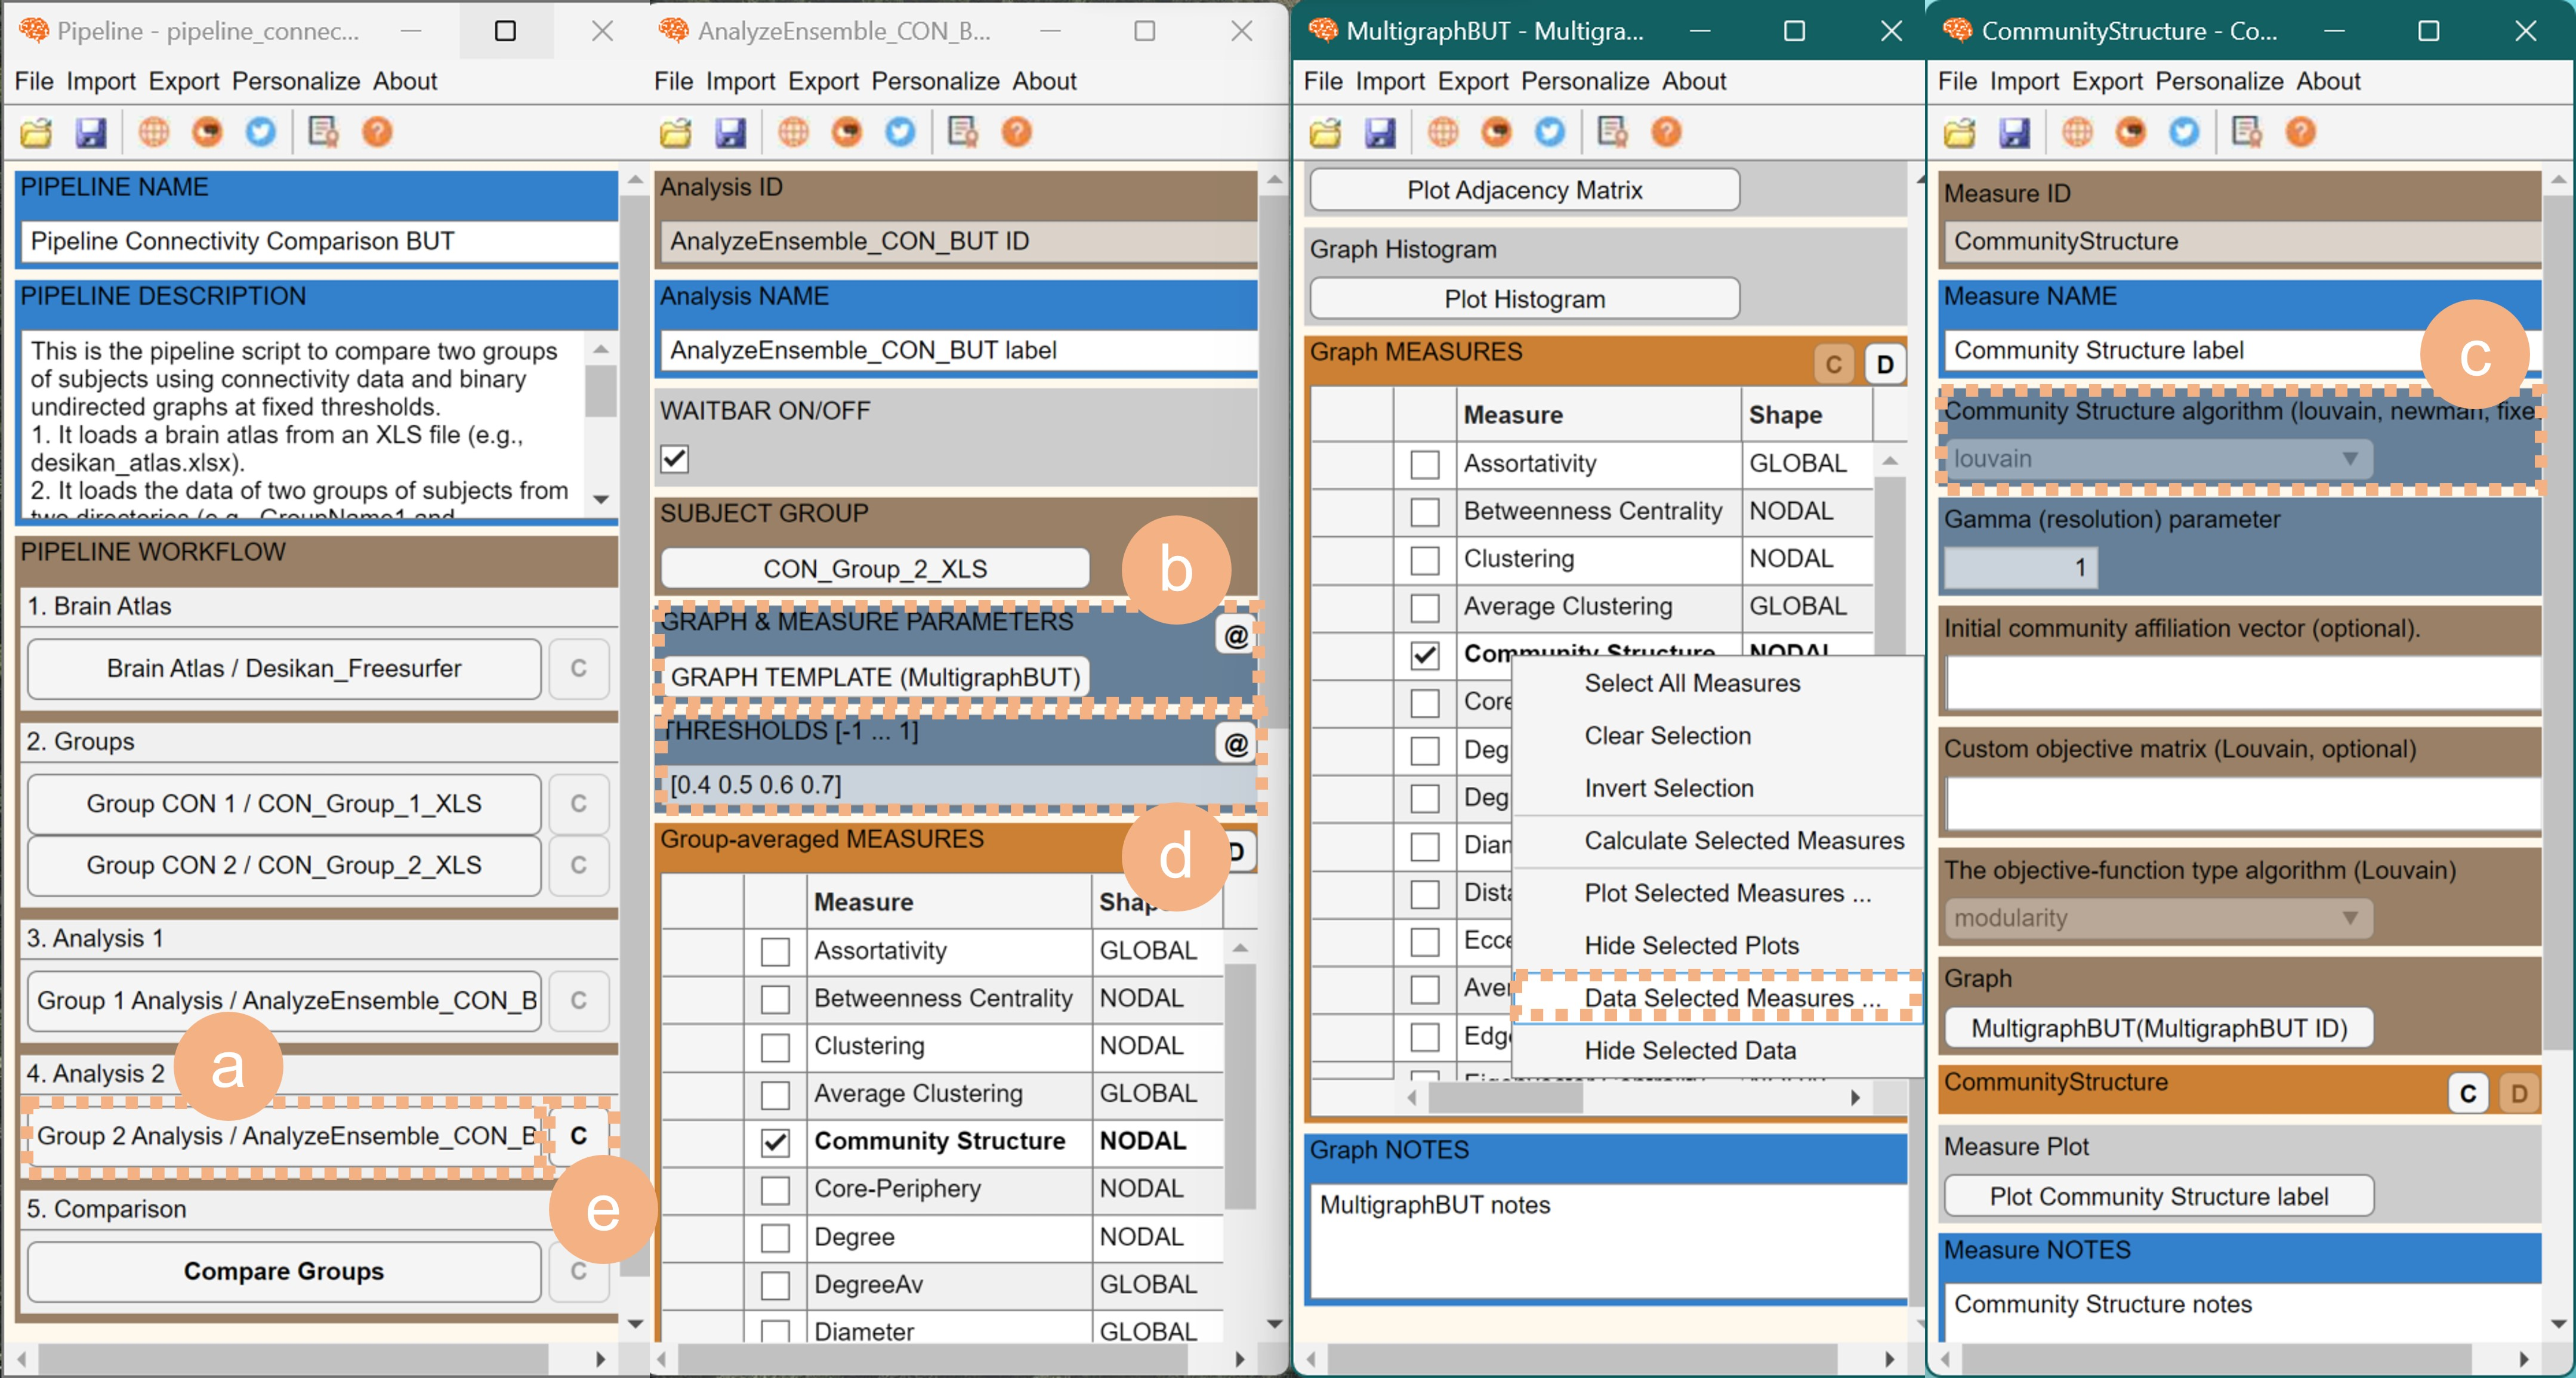
\includegraphics{fig06.jpg}
	}
	{Parameters blocked in Analysis of Group 2}
	{
	{\bf a} Click on \fn{Analysis 2} in the pipeline's GUI.
	{\bf b} In this new window, you can see that the measure parameters, such as the {\bf b} \fn{GRAPH TEMPLATE} and {\bf c} rule for \fn{Community Structure}, as well as the graph property, such as the {\bf d} \fn{THRESHOLDS}, are blocked since they are intended to be the same as the ones set in the analysis of group 1. You have the flexibility to reset the analysis parameters for Group 1 by clicking on the checkbox marked with a 'C' next to the settings of Group 1 {\bf e}.
	}
 
\section{Step 5: Comparing Groups}

After thoroughly exploring the network measures for each group, it's time to move on to their statistical comparison. To initiate this process, click on \fn{Compare Groups} (\Figref{fig:07}a).

In the new window, you have several options to configure the analysis according to your research needs. First, you can choose whether to enable a progress bar and verbose functions while the analysis is running. This can help you monitor the progress of the analysis. You can also specify how many permutations you want to use to assess differences between groups (\Figref{fig:07}b).

If your groups are not independent and represent the same subjects at different points in time, you can select the longitudinal comparison option. This option will permute the values within each subject, considering their temporal relationship (\Figref{fig:07}b).

For computational efficiency during this tutorial, we've set the number of permutations to 10. However, for your research analysis, we recommend using a more extensive number, such as 1000 or 10000 permutations, to ensure robust results.

Next, you can select the specific graph measures you wish to compare between the groups. To do this, click on “C” in the \fn{COMPARISONS} section (\Figref{fig:07}c). Once you've chosen all the measures of interest, right-click and select \fn{Calculate Selected Comparisons}.

If you've enabled the progress bar and verbose functions, two additional windows will appear to display the progress of the comparison calculations. Finally, there's an option in this GUI to save intermediate results during the permutations, which can be helpful for further analysis.

	\fig{figure}
	{fig:07}
	{
	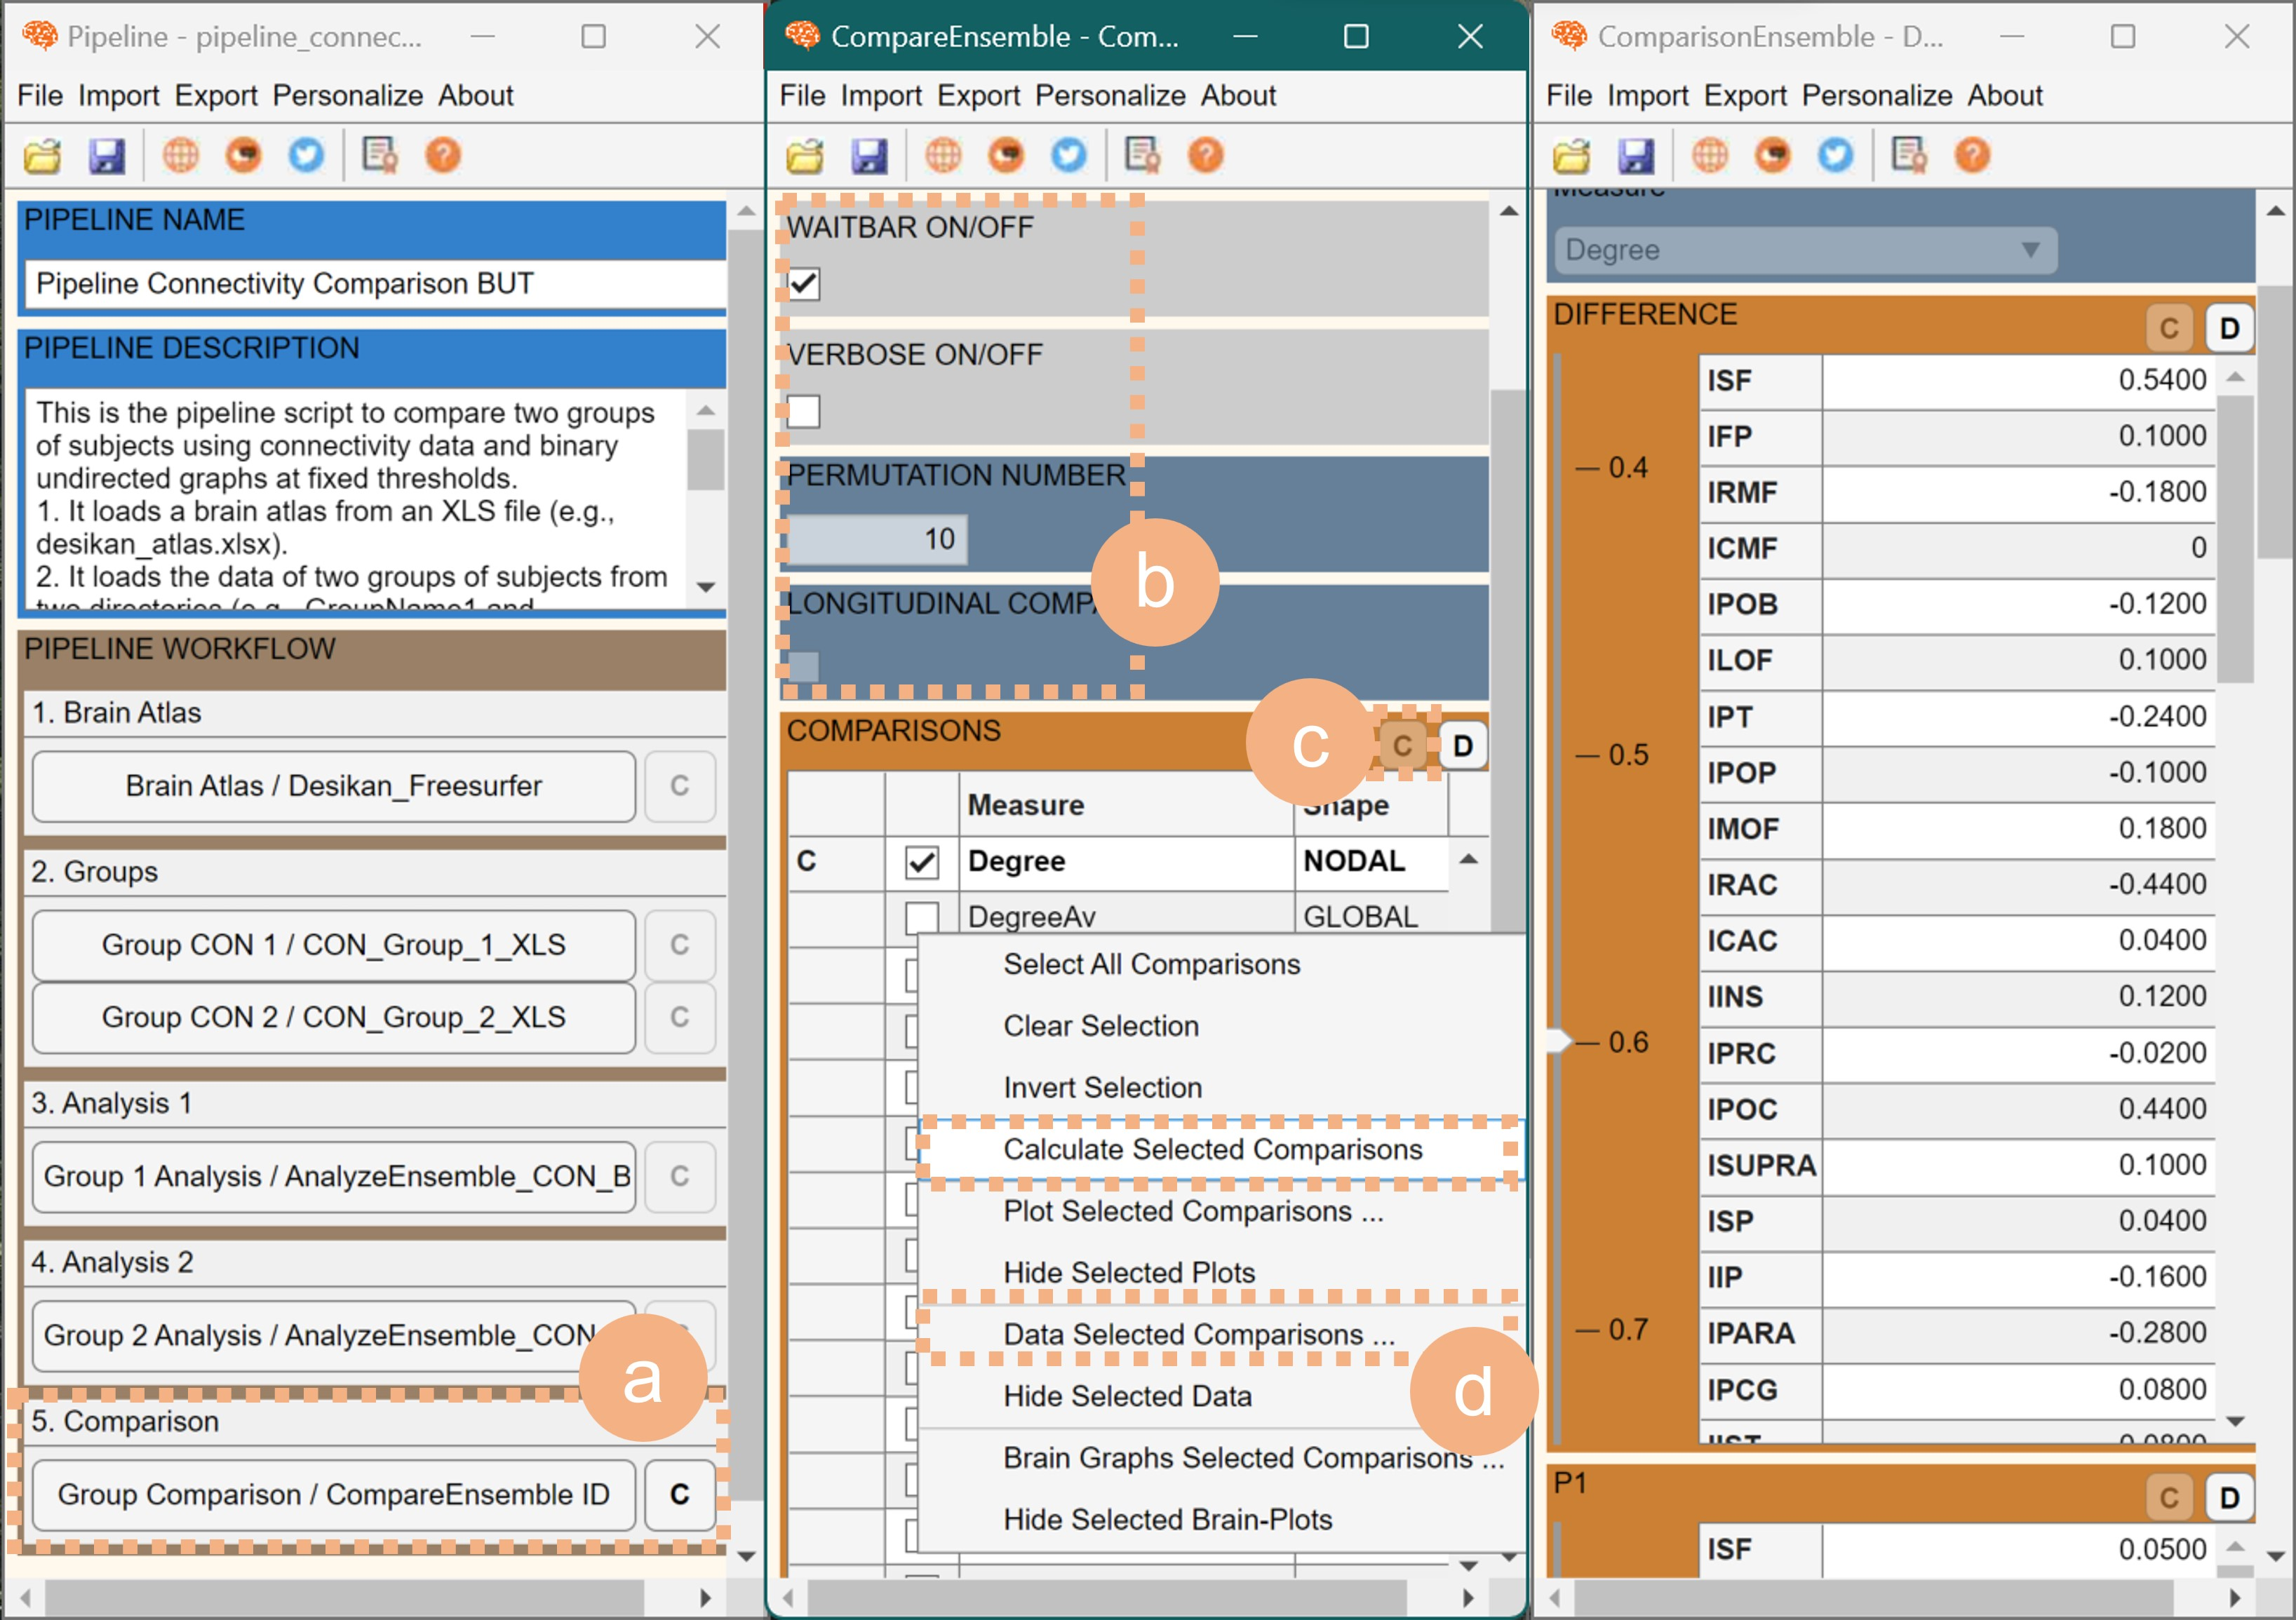
\includegraphics{fig07.jpg}
	}
	{Compare the Group Data}
	{
	{\bf a} Click on \fn{Compare Groups} in the pipeline's GUI.
	{\bf b} In this new window, you can select what to turn ON/OFF the wait bar and verbose functions, you can change the number of permutations, and whether to perform a longitudinal group comparison. We set the number of permutations to 10 for this tutorial {\bf c}. Finally, you can calculate the comparison of some graph measures between groups {\bf d}.
	}
 
To obtain the results from the measure's comparison, select the measures in the \fn{COMPARISONS} panel and press \fn{Data Selected Comparisons}({\Figref{fig:07}d}), and a new window will open where we can check the difference value between groups, the p-values (1-tailed and 2-tailed), as well as the confidence intervals.

 	\fig{figure}
	{fig:08}
	{
	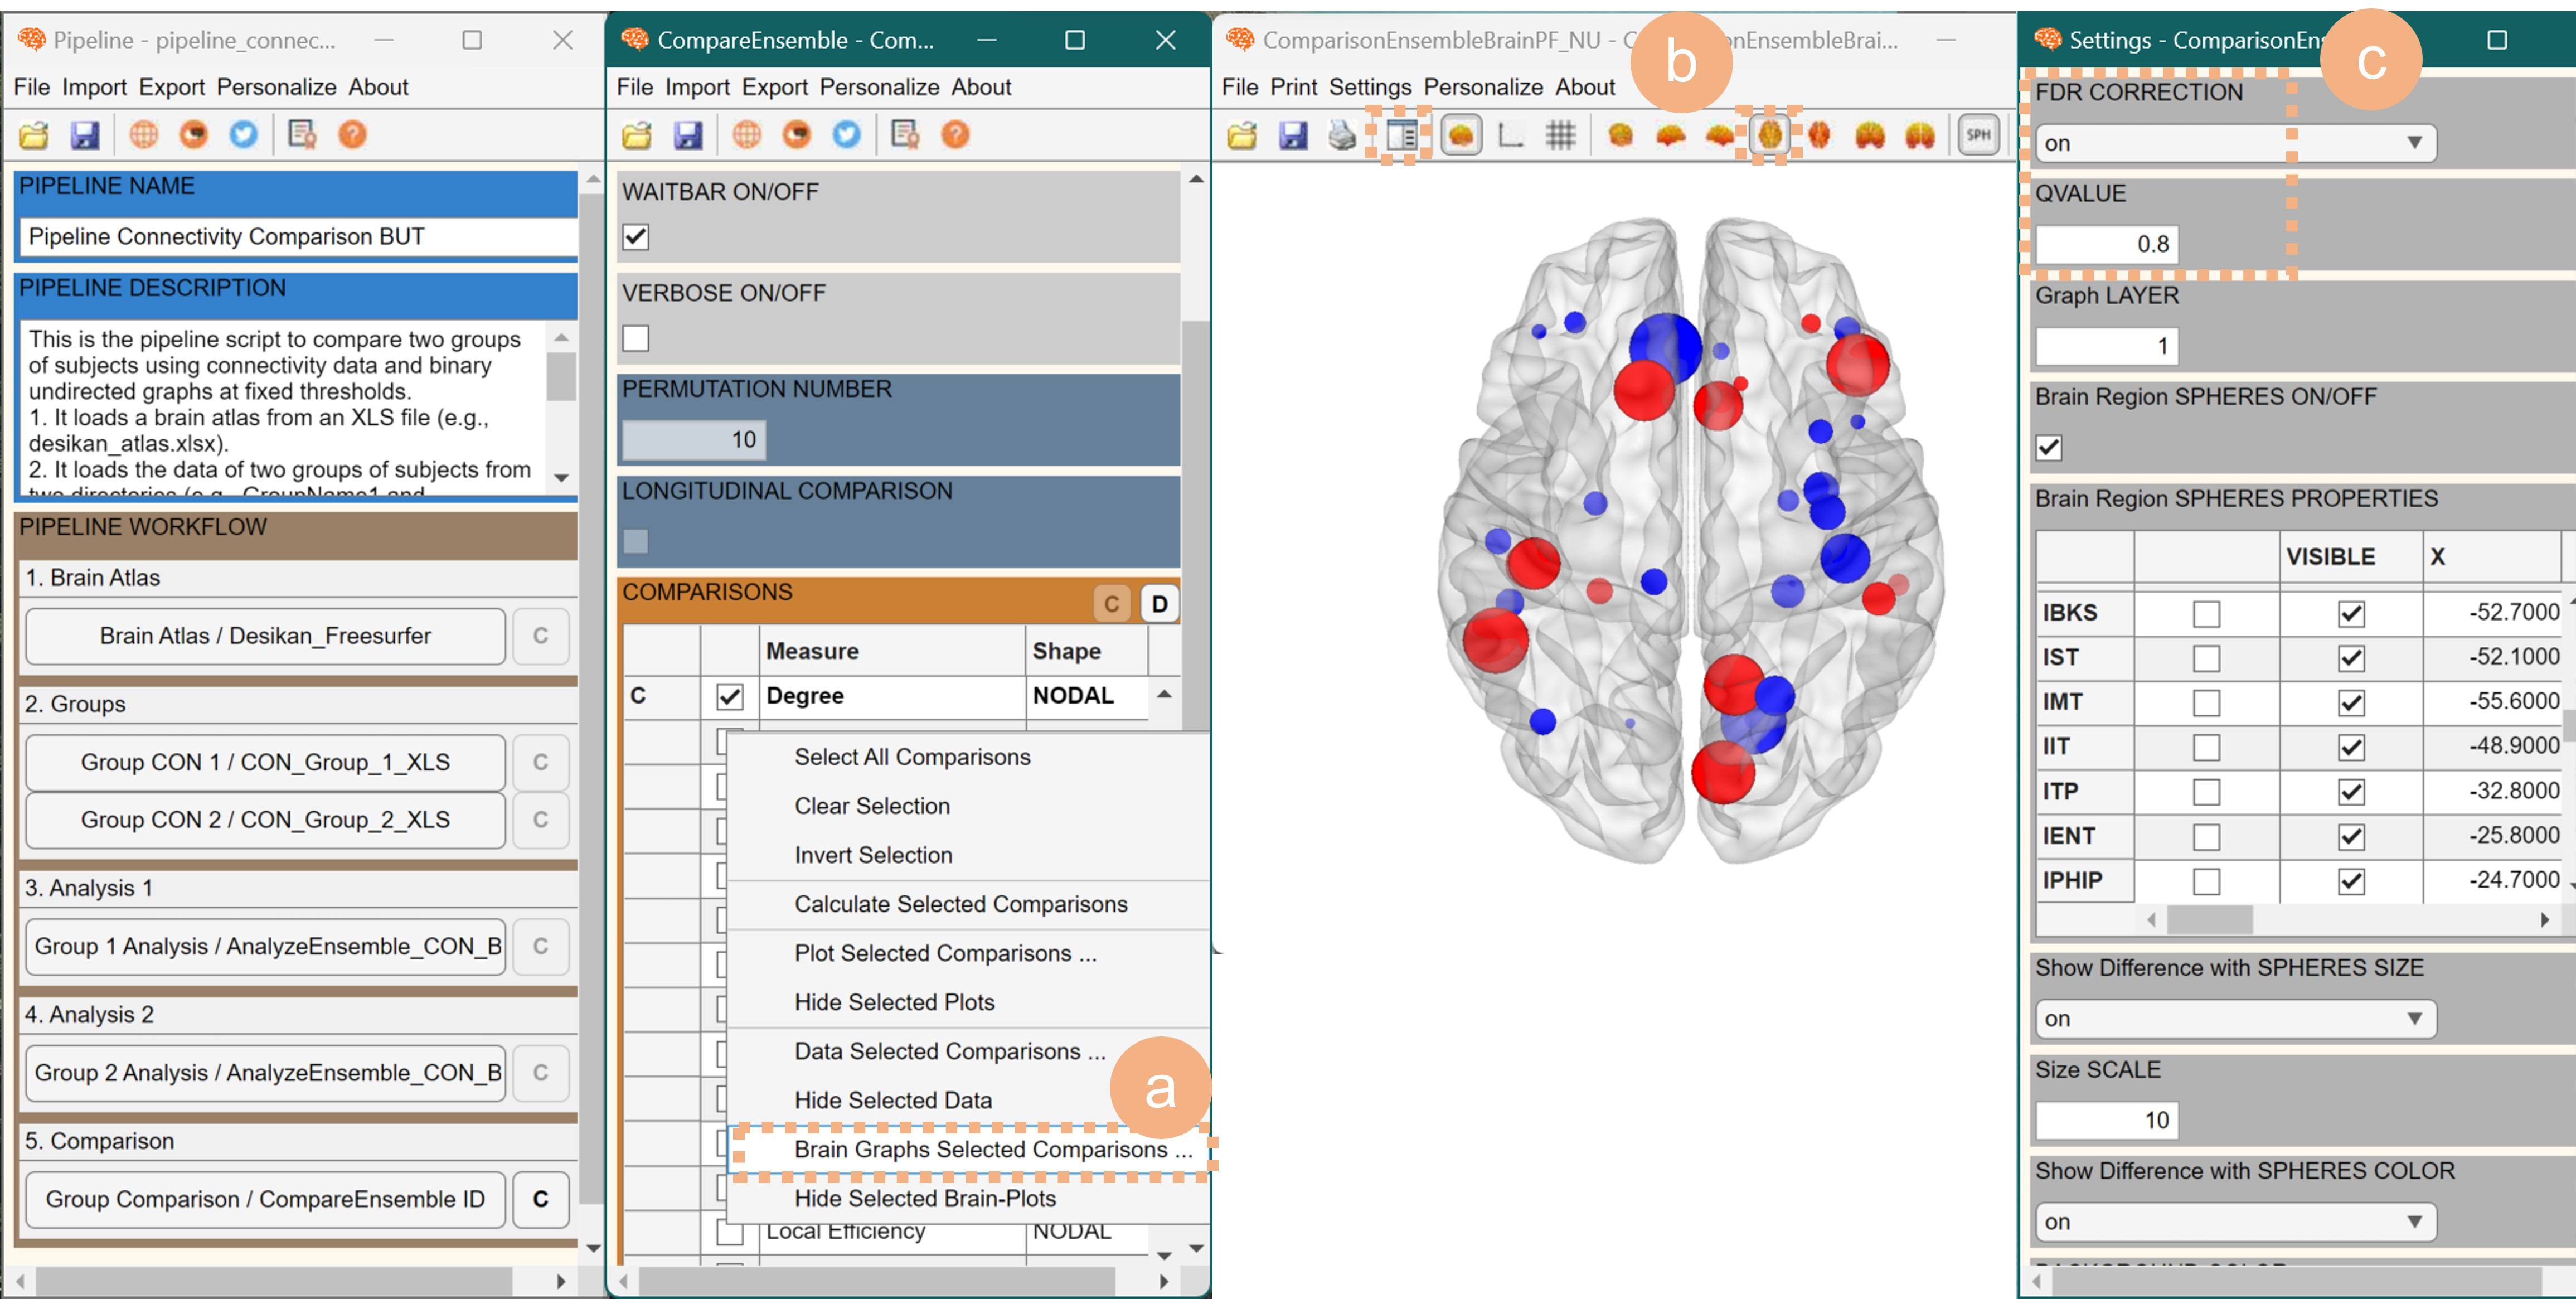
\includegraphics{fig08.jpg}
	}
	{Visualize the comparison results in a brain surface}
	{
	{\bf a} Click on \fn{Brain Graph Selected Comparison} in the Comparisons panel.
	{\bf b} In this new window, you'll see the comparison results, with positive values in red and negative values in blue on the brain surface.
{\bf c} You can customize and save plot visualizations within the settings menu.
	}

If you wish to visualize the results, simply right-click at the top of the table and select \fn{Brain Graph Selected Comparison} within the Compare Ensemble interface (\Figref{fig:08}a). This action will open a brain surface displaying the difference between these two groups in terms of the \fn{Degree} data.

Within the brain surface interface's toolbar, you have various options to explore. For example, by clicking on the “Axial dorsal” button (\Figref{fig:08}b), you can access the same view depicted in \Figref{fig:08}. Additionally, the “Settings Panel Figure” button in the same toolbar allows you to fine-tune different visualization settings.

For further customization, within the settings menu (\Figref{fig:08}c), you can activate the \fn{FDR CORRECTION} feature to control for multiple comparisons and reduce the likelihood of obtaining false positive results when assessing the significance of connectivity measures across multiple brain regions. You can also utilize the settings menu to personalize the visualization of your plots and save them for future reference.

\end{document}